\chapter{Evaluation des besten Lösungsansatzes}
\label{ch:evaluation-loesungsansatz}

Aufbauend auf den beiden vorangegangenen Kapiteln, in denen Lösungsansätze entworfen und die Implementierung
beschrieben wurde, konnte ein Vorgehen zur Auswahl der besten \ac{KI}-Strategie entwickelt werden, auf die in diesem
Kapitel eingegangen wird.

\section{Vorgehen zur Auswahl der besten Strategie}
\label{sec:auswahl-strategie}

Die Überlegung hierbei war es, basierend auf der in \Kapitel{sec:offline-implementierung} beschriebenen
Möglichkeit, Spiele auch ohne Zugriff auf den spe\_ed-Server mit mehreren unserer \ac{KI}s ausführen zu können,
eine automatisierte Simulation möglichst vieler Spiele durchführen zu können.
Die daraus resultierenden Ergebnisse sollten in einer Form gespeichert werden, die es im Anschluss ermöglicht, daraus
Informationen über die Stärke einer bestimmten \ac{KI} mit ihren unterschiedlichen Konfigurations-Möglichkeiten gewinnen
zu können. \\

Zu diesem Zweck wurde die Klasse \Code{AIEvaluationController} erstellt, der vom bereits erläuterten
\Code{OfflineController} erbt.
Dieser ruft bei der Ausführung in einer Schleife die \Code{play}-Methode des \Code{OfflineController} auf, wobei bei
jedem Aufruf ein neues Spiel generiert wird.
Hierbei mussten allerdings einige Annahmen getroffen werden, die potentiell einen Einfluss auf das Ergebnis haben
könnten:

\begin{itemize}
    \item Ein Spielfeld besitzt bei der Simulation eine zufällige Höhe und Breite zwischen 30 und 70 Feldern.
    \item Den \ac{KI}s wird für die Auswahl in einer Runde eine zufällige Zeit zwischen 3 und 15 Sekunden eingeräumt.
    \item Es nehmen an einem Spiel immer eine zufällige Anzahl an Spielern teil, die zwischen 3 und 6 liegen kann.
\end{itemize}

Nach jeder Berechnung einer \ac{KI} wird die Berechnungsdauer abgespeichert.
Gleiches wird nach dem Ende eines jeden Spiels für das Spiel selber und die teilnehmenden Spieler durchgeführt, wobei
auch die Information über den Sieger eines Spiels erhalten bleibt.

\section{Entwurf einer \acL{DB} zum Speichern der Simulationen}
\label{sec:entwurf-datenbank}

Um die beschriebenen Daten leicht abfragen zu können, fiel die Entscheidung auf die Nutzung einer relationalen
\ac{DB}.
In diesem Fall wurde dafür SQLite3 ausgewählt, da die gesamte \ac{DB} in einer Datei gespeichert wird und somit das
Aufsetzen eines \acl{DB}-Managements-Systems entfällt. \Vgl{sqlite3}
Die Verbindung konnte dann mit der Python-Bibliothek \Code{sqlite3} \Vgl{python-sqlite3} hergestellt werden.
Zuerst aber war es notwendig, die \ac{DB}-Struktur zu entwerfen, um anschließend entsprechende SQL-Statements im Code
auf die \ac{DB} anwenden zu können.

\subsection{Erstellen des \acl{ER}-Modells}
\label{subsec:er-modell}

Das Vorgehen zum Entwerfen einer \ac{DB}-Struktur war uns aus dem Modul Informationssysteme I, das an der Universität
Oldenburg von \href{https://uol.de/is/personen/mitarbeiter/ralf-krause}{Ralf Krause} und
\href{https://uol.de/marcograwunder}{Marco Grawunder} angeboten wird, bekannt.
Im ersten Schritt wurde dazu ein \ac{ER}-Modell basierend auf den zugrunde liegenden Anforderung entworfen.
Wie bereits beschrieben, wollen wir primär Informationen erhalten, wie oft eine
bestimmte \ac{KI} mit welchen Parametern in den simulierten Spielen gewonnen hat.
Ein weiterer wichtiger Wert stellt die durchschnittliche Ausführungsdauer einer \ac{KI} dar und diesen \ua
mit der Spielfeldgröße und der Anzahl der am Spiel teilnehmenden Gegnern in Korrelation bringen zu können.
Das daraus resultierende \ac{ER}-Modell ist in \Abbildung{fig:er-schema} dargestellt.

\begin{figure}[htb]
	\centering
	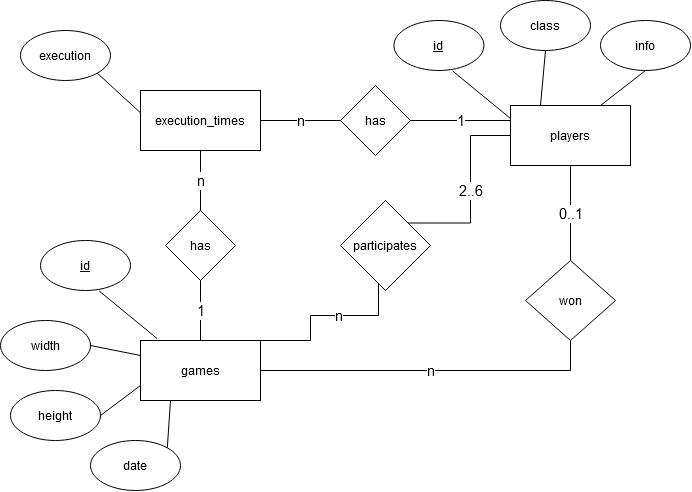
\includegraphics[width=0.7\textwidth]{Bilder/er-diagram.png}
	\caption{\ac{ER}-Modell der Evaluations-\ac{DB}}
	\label{fig:er-schema}
\end{figure}

\subsection{Überführung in ein relationales \acl{DB}-Modell}
\label{subsec:db-schema}

Dieses Modell wurde dann anschließend in ein relationales Modell überführt, welches die tatsächlichen Relationen in der
Datenbank darstellt.
Dazu wurden Primärschlüssel festgelegt und über Fremdschlüssel Verknüpfungen zwischen den Relationen hergestellt.
Bei der Modellierung wurde darauf geachtet, die dritte Normalform der \ac{DB}-Normalisierung einzuhalten.
\Vgl{db-normalisierung}
In \Abbildung{fig:relationales-db-schema} ist das entworfene relationale Modell zu sehen.

\begin{figure}[htb]
	\centering
	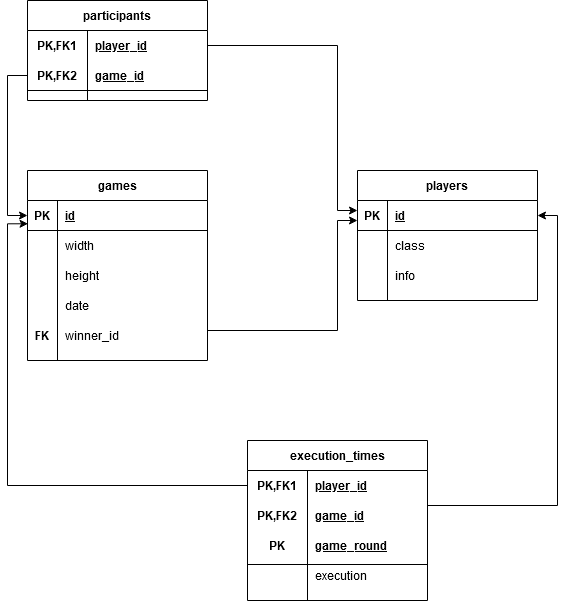
\includegraphics[width=0.5\textwidth]{Bilder/relationales_db_schema.png}
	\caption{Relationales Datenbankschema der Evaluations-Datenbank}
	\label{fig:relationales-db-schema}
\end{figure}

\section{Ergebnis der Evaluation}
\label{sec:ergebnis-evaluation}

\todo{Kapitel schreiben}
